\documentclass[10pt,a4paper]{article}
\usepackage[utf8]{inputenc}
\usepackage[english]{babel}
\usepackage[T1]{fontenc}
\usepackage{geometry}
\geometry{left=1.5cm, right=1.5cm, top=1.5cm, bottom=1.5cm}
\usepackage{graphicx}
\usepackage{xcolor}
\usepackage{hyperref}
\usepackage{enumitem}
\usepackage{titlesec}

% Color Palette Definitions
\definecolor{darkblue}{HTML}{1A365D}
\definecolor{primaryblue}{HTML}{2B6CB0}
\definecolor{darkgray}{HTML}{2D3748}
\definecolor{lightgray}{HTML}{EDF2F7}

\hypersetup{
    colorlinks=true,
    linkcolor=primaryblue,
    urlcolor=primaryblue,
    pdftitle={Sándor Hatalovics CV},
    pdfpagemode=FullScreen,
}

% Heading Formatting
\titleformat{\section}{\large\bfseries\color{darkblue}}{}{0em}{}[\titleline{\color{primaryblue}}]
\titlespacing{\section}{0pt}{10pt}{6pt}

\setlist[itemize]{leftmargin=12pt, noitemsep, topsep=2pt}

\begin{document}
\pagestyle{empty}

% HEADER (Name, Title, Contact Info & Photo)
\begin{minipage}[t]{0.75\textwidth}
    {\Huge\bfseries\color{darkblue} SÁNDOR HATALOVICS} \\[4pt]
    {\large\bfseries\color{primaryblue} Business Informatics \& Computer Science Student | Full-Stack Web Developer} \\[8pt]
    \begin{tabular}{ll}
        \textbf{Email:} \href{mailto:sandorhatalovics@gmail.com}{sandorhatalovics@gmail.com} & \textbf{GitHub:} \href{https://github.com/Szasa-24}{github.com/Szasa-24} \\
        \textbf{Phone:} +36 30 798 2251 & \textbf{Availability:} 100\% Remote (Home Office) \\
        \textbf{Schedule:} Part-Time (up to 30 hours/week) &
    \end{tabular}
\end{minipage}
\begin{minipage}[t]{0.23\textwidth}
    \raggedleft
    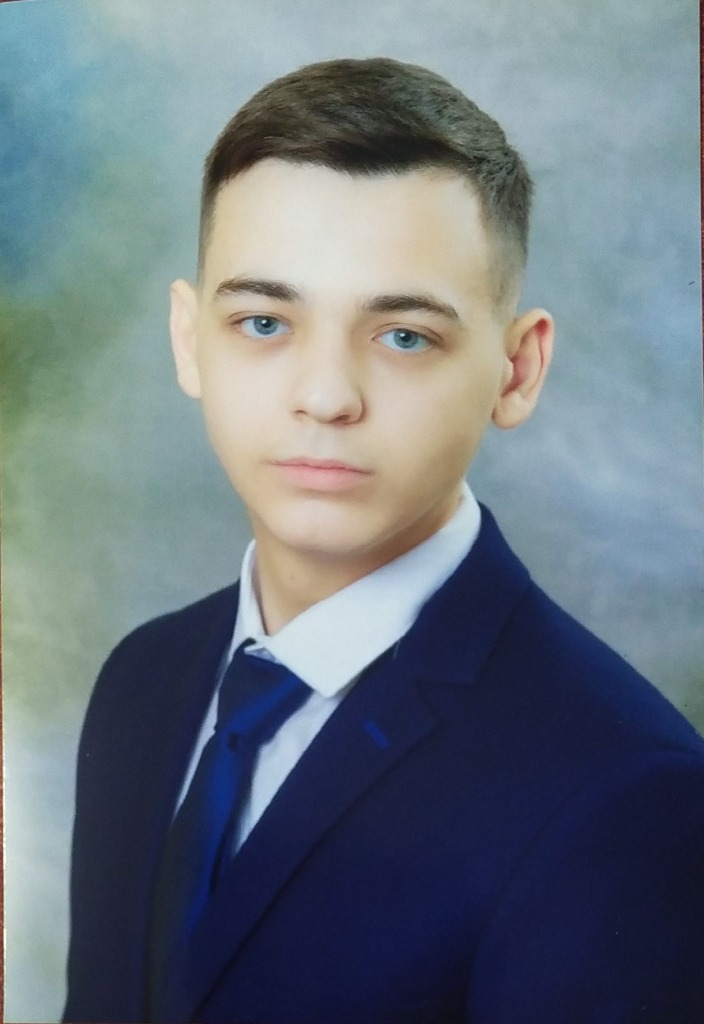
\includegraphics[width=2.8cm,height=3.5cm,keepaspectratio]{profile.jpg}
\end{minipage}

\vspace{10pt}

% PROFESSIONAL SUMMARY
\section{Professional Summary}
{\color{darkgray}
Highly motivated Computer Science and Business Informatics double major student with a strong passion for modern web engineering. Experienced in building full-stack web applications from scratch using Next.js, TypeScript, PostgreSQL, and Firebase. Proven ability to work independently in remote environments, write clean and maintainable code, and quickly learn new frameworks and technologies.
}

% FEATURED PROJECTS
\section{Featured Projects}

\textbf{1. Franklin Photo -- Premium Client Gallery \& Admin Dashboard} \hfill \href{https://franklin-photo.vercel.app/}{franklin-photo.vercel.app}
\begin{itemize}
    \item \textbf{Description:} A complete, secure client-facing gallery portal and photographer management panel designed for school events (e.g., graduation ceremonies) and private photo sessions. Photographers can manage school directories and bulk upload high-resolution images via a protected admin dashboard. Clients log in using unique secure codes to view, select, and download their complete photo portfolios using a server-side ZIP compilation stream.
    \item \textbf{Tech Stack:} Next.js 15 (App Router), React 19, TypeScript, TailwindCSS v4, Motion (animations), PostgreSQL, Drizzle ORM, Firebase Auth, Firebase Admin SDK, Vercel Blob Storage, Node.js (\texttt{archiver}, \texttt{busboy}).
    \item \textbf{Code:} \href{https://github.com/Szasa-24/franklin-photo}{github.com/Szasa-24/franklin-photo}
\end{itemize}

\vspace{6pt}

\textbf{2. Hatalyx Studio Web} \hfill \href{https://github.com/Szasa-24/hatalyx-studio-web}{github.com/Szasa-24/hatalyx-studio-web}
\begin{itemize}
    \item \textbf{Description:} A high-end, responsive agency portfolio website with smooth scroll animations. Built with a full translation architecture (Hungarian/English) utilizing React Context API to ensure instant, client-side language switching.
    \item \textbf{Tech Stack:} Next.js (App Router), React, TypeScript, TailwindCSS, Motion, React Context API.
\end{itemize}

% TECHNICAL SKILLS
\section{Technical Skills}
\begin{itemize}
    \item \textbf{Frontend:} Next.js (App Router), React, TypeScript, JavaScript (ES6+), TailwindCSS (v4), CSS3, HTML5, Responsive UI/UX Design, Figma (UI/UX layouts).
    \item \textbf{Backend \& API:} Node.js (Next.js API Routes / Route Handlers), Firebase Admin SDK, REST API Design, JWT (JSON Web Tokens), BcryptJS (encryption).
    \item \textbf{Databases:} PostgreSQL, Drizzle ORM, SQL, Relational Database Design, Query Optimization.
    \item \textbf{DevOps \& Tools:} Git / GitHub, Vercel, Firebase Console, Unix-based systems (FreeBSD), Terminal/CLI, LaTeX.
    \item \textbf{Programming Languages:} TypeScript, JavaScript, Python, C++.
\end{itemize}

% EDUCATION
\section{Education}
\textbf{University of Miskolc} \hfill 2025 -- Present
\begin{itemize}
    \item B.Sc. in Business Informatics (Gazdaságinformatikus)
\end{itemize}
\vspace{4pt}
\textbf{Ferenc Rákóczi II Transcarpathian Hungarian College (Berehove)} \hfill 2025 -- Present
\begin{itemize}
    \item B.Sc. in Computer Science (Informatika), part-time/correspondence program
\end{itemize}

% KEY COMPETENCIES
\section{Key Competencies}
\begin{itemize}
    \item \textbf{Full-Stack Mentality:} Comfortable managing the entire lifecycle of an application, from database design and API development to frontend animations and polish.
    \item \textbf{Self-Motivation \& Independence:} Capable of working autonomously, debugging complex issues, and architecting solutions without supervision—ideal for remote team collaboration.
    \item \textbf{Technical English:} Fluent in reading and writing technical documentation. Actively practicing and improving spoken conversational English.
\end{itemize}

\end{document}
